\documentclass[10pt,a4paper]{article}
\usepackage[utf8]{inputenc}
\usepackage[francais]{babel}
\usepackage[T1]{fontenc}
\usepackage{amsmath}
\usepackage{amsfonts}
\usepackage{amssymb}
\usepackage{graphicx}
\usepackage{envmath}
\usepackage[left=2cm,right=2cm,top=2cm,bottom=2cm]{geometry}
\usepackage{ulem}
\usepackage{moreverb}
\usepackage{framed}
\usepackage{listings}
\usepackage{mathenv}
\usepackage{color}
\usepackage{eurosym}
\usepackage{float}

\title{Correction orthographique par apprentissage Bayésien}
\author{Edouard \textsc{Leurent} \\ Bastien \textsc{Debras}}

\definecolor{dkgreen}{rgb}{0,0.6,0}
\definecolor{gray}{rgb}{0.5,0.5,0.5}
\definecolor{mauve}{rgb}{0.58,0,0.82}

\lstset{language=Java, numbers=left, frame = single, keywordstyle = \color{blue}, commentstyle=\color{dkgreen} , numberstyle=\tiny\color{gray}, rulecolor=\color{black}, stringstyle=\color{mauve}, breaklines=true,   title=\lstname}



\begin{document}


\maketitle

\begin{center}

\includegraphics[width=0.2\textwidth]{logo_mines}\\ 
\Large{Cours d'apprentissage artificiel}
\end{center}
\setcounter{tocdepth}{3}
\tableofcontents
\vspace{5cm}

\newpage

\section{Introduction}
\subsection{Démarche}
Comment réagir face à une faute d'orthographe ? Une première idée pourrait être de regarder dans un \textbf{dictionnaire}. Si l'utilisateur tape un mot qui ne fait pas partie du dictionnaire, on le remplace simplement par le mot du dictionnaire le plus proche (en un sens à préciser). 

Cependant, on se rend vite compte que cette définition du mot "le plus proche" est ambigüe : que faire si un grand nombre de mots sont tous également candidats à être le mot le plus proche ?

Dans cette situation, notre démarche pour lever l'ambiguïté a été de choisir mot le plus \textbf{probable}, c'est à dire le plus fréquent, celui qui apparait le plus dans l'usage. Pour apprendre ces fréquences, il faut donc disposer non pas d'un simple dictionnaire, mais plutôt d'un \textbf{corpus} de textes.

\section{Formalisation}

Nous allons ici préciser nos problèmes, et expliquer notre choix d'algorithmes pour les traiter

\subsection{Les problèmes}
Nous allons voir que le problème de correction orthographique peut se ramener à un problème de Machine Learning.\\
\begin{itemize}
\item On considère un mot tapé par l'utilisateur comme une \textbf{observation} du mot réel qu'il a voulu écrire. Les mots d'une langue sont alors interprétées comme des \textbf{classes}. Corriger une faute d'orthographe revient donc à trouver à quelle classe appartient une observation donnée. Nous avons un \textbf{premier problème de classification}, très fortement multiclasse (par exemple, la langue française contient environ 100 000 mots).
\item Pour rester général, nous avons décider de ne pas considérer uniquement le français mais de traiter le cas d'un \textbf{langage quelconque}. Une fois plusieurs langages appris, corriger une phrase donnée nécessite de savoir dans quel langage il faut raisonner. On doit donc être capable d'identifier dans quelle langue est écrite une phrase donnée. La détection de la langue constitue alors notre \textbf{deuxième problème de classification}.
\end{itemize}

Pour nos exemples, nous avons choisi d'utiliser le français et l'anglais.

\subsection{Méthode Bayésienne}
On a choisit de considérer les mots les plus probables, et on a donc adopté une approche probabiliste. Une méthode adéquate est donc d'utiliser un \textbf{classifieur naïf de Bayes}.\\

Il est formalisé de la manière suivante :\\

Étant donné l'ensemble $C$ des corrections possibles  d'un mot donné, on s'intéresse à la probabilité qu'une correction particulière soit la bonne.\\

\begin{array}{l l}
$On note$ &m $ le mot tapé par l'utilisateur$\\
	&c $ une correction possible de ce mot$ \\
	&P(c|m) $ la probabilité que le mot lu $m$ soit une observation du mot correct $c
\end{array}\\

On a alors, d'après la \textbf{formule de Bayes}

\begin{equation}
P(c|m) = \frac{P(m|c) \bullet P(c)}{P(m)}
\end{equation}

On essaie de maximiser cette quantité. Le dénominateur $P(m)$ n'est donc qu'un facteur normalisateur qui est constant sur l'ensemble $C$ des corrections, et on peut donc choisir la convention $P(m) = 1$\\

On cherche donc 

\begin{equation}
\max\limits_{c \in C} P(m|c) \bullet P(c)
\end{equation}

On constate alors que notre fonction à maximiser est constituée de deux termes\\

\begin{itemize}
\item $P(m|c)$ la probabilité d'avoir fait la faute $m$ en voulant taper le mot $c$. C'est le \textbf{modèle d'erreur}.
\item $P(c)$ la probabilité que l'utilisateur ait voulu taper le mot $c$. C'est le \textbf{modèle de langage}.\\
\end{itemize}

Cette séparation en deux termes est très intuitive. Comment corriger la faute de frappe \textit{histre} par exemple ? On peut proposer les deux corrections \textit{bistre} et \textit{histoire} par exemple. Laquelle est la meilleure ?\\

\begin{itemize}
\item D'un coté la mot \textit{bistre} est plus proche de \textit{histre} que la mot \textit{histoire}, car une seule modification est nécessaire contre deux pour \textit{histoire}. Il est plus probable que l'utilisateur ait faite une seule faute plutôt que deux fautes dans un même mot.
\item D'un autre coté, le mot \textit{histoire} est bien plus courant que le mot \textit{bistre}, et il est donc plus probable que l'utilisateur ait voulu écrire ce mot.\\
\end{itemize}

Il faut donc bien considérer ces deux critères du modèle de langage et du modèle d'erreur pour pouvoir lever l'ambiguïté et choisir la meilleure correction.

\subsection{Le modèle de langage}

Il nous faut établir un modèle permettant d'évaluer la probabilité $P(c)$ qu'un mot $c$ soit utilisé.

Pour cela, on aborder une approche pragmatique : plus on rencontre un mot dans le corpus des textes, plus sa probabilité sera grande. La probabilité du mot est donc déterminée par sa fréquence.
En fait, on assimile directement la probabilité d'un mot au nombre de ses occurrences. On ne divise pas par le nombre de mots du corpus, qui ne constitue qu'un facteur multiplicatif et ne permet pas de différencier les différentes corrections.

On pose donc simplement

\begin{equation}
P(c) = \#\{\text{occurences de }c\}
\end{equation}

\subsection{Le modèle d'erreur}

On doit mettre en place un modèle permettant de calculer $P(m|c)$, la probabilité qu'en voulant écrire $c$ l'utilisateur fasse une ou plusieurs fautes et aboutisse au mot $m$.

Nous avons choisit un modèle simple, basé sur la notion d'\textbf{opération élémentaire}.

Une opération élémentaire sur un mot est définie comme étant au choix : \\

\begin{itemize}
\item La suppression d'une lettre du mot
\item Le remplacement d'une lettre du mot
\item L'insertion du lettre dans le mot
\item La transposition de deux lettres du mot
\end{itemize}

On interprète alors une faute de frappe comme une opération élémentaire, à laquelle on attribue une certaine probabilité d'erreur $P_e$. Cette probabilité est un paramètre de l'algorithme, choisi ici à $1/20^{\text{ème}}$.\\

On calcule ensuite la distance d'édition $d$ entre deux mots, c'est à dire le nombre minimal d'opérations élémentaires pour passer d'un mot à l'autre.

On pose finalement le modèle d'erreur suivant : 

\begin{equation}
P(m|c) = {P_e}^{d(m,c)}
\end{equation}

Chaque opération élémentaire effectuée diminue donc la probabilité d'un facteur $P_e$.

\subsection{Détection de la langue}

On cherche la probabilité $P(l|m_1m_2m_3...m_n)$ qu'une phrase formée de plusieurs mots $m_1$ $m_2$ $m_3$ ... $m_n$ soit écrite en une langue $l$.
 
 Cette probabilité s'exprime à nouveau par la \textbf{formule de Bayes}

 \begin{equation}
 P(l|m_1m_2m_3...m_n) = \frac{P(m_1m_2m_3...m_n|l)P(l)}{P(m_1m_2m_3...m_n)}
 \end{equation}
 
 Examinons chacun de ces termes
 
 \begin{itemize}
 \item $P(m_1m_2m_3...m_n)$ est la probabilité de la phrase. Ce terme est difficile à évaluer et est un facteur multiplicatif constant indépendant de les langues qu'on est en train de comparer. On peut donc sans perte de généralité le choisir comme égal à 1.
 \item $P(l)$ représente la probabilité de la langue. On suppose ici que l'utilisateur tape une phrase en français ou en anglais de manière équivalente, et on suppose alors toutes les langues équiprobables. A nouveau, ce terme est choisi comme étant égal à 1.
 \item $P(m_1m_2m_3...m_n|l)$ est la probabilité de la phrase sachant qu'elle est écrite en français. Pour simplifier le calcul, on prend une \textbf{hypothèse très forte} : on suppose les mots \textbf{indépendants} deux a deux. Ce n'est pas du tout le cas en pratique, ne serait-ce qu'à cause des règles de grammaire et des expressions idiomatiques, mais cela est suffisant pour avoir une bonne approximation. En effet, ce terme s'exprime alors 
\begin{equation}
P(m_1m_2m_3...m_n|l) = P(m_1|l) \times P(m_2|l) \times P(m_3|l) \times ... \times P(m_n|l) = \prod_{i=1}^nP(m_i|l)
\end{equation}

Or, les termes $P(m_i|l)$ peuvent être obtenus de la même manière que $P(c)$ précédemment, directement par le nombre d'occurrences dans le modèle de langage.\\
 \end{itemize}
 
 On a donc finalement l'équation suivante : 
 \begin{equation}
P(l|m_1m_2m_3...m_n) = \prod_{i=1}^nP(m_i|l)
 \end{equation}

\section{Implémentation}

Nous avons implémenté le modèle formel présenté ci-dessus dans un programme en Java. Nous décrirons chaque partie de notre code-source en suivant le plan du modèle.

\subsection{Modèle de langage}
\subsubsection{La structure de dictionnaire}
\label{tyrannosaure}

On veut stocker le nombre d'occurrences de chaque mot des œuvres du corpus. La structure de données que nous avons choisi est une table de hachage, implémentée en Java selon l'interface \verb!Map! et la classe \verb!HashMap!.

On se pose alors la question suivante : que faire si l'on rencontre un mot tel que \textit{tyrannosaure}, parfaitement français mais jamais lu dans notre corpus d'apprentissage ? Il ne serait pas raisonnable de lui affecter une probabilité nulle uniquement parce qu'on ne l'a jamais vu auparavant. Il y a plusieurs approches possibles de ce problème, et nous avons décidé d'appliquer la plus simple d'entre elle : traiter un nouveau mot comme si on l'avait déjà vu une seule fois. Ce procédé s'appelle le \textbf{lissage}, parce qu'on lisse la distribution de probabilités qui aurait été nulle, l'arrondissant au plus petit dénombrement possible.

Pour cela, nous avons modifié légèrement la classe \verb!HashMap! de la manière suivante : quand on fait un appel à la fonction \verb!get()! et que la clé requise n'est pas présente dans la table de hachage, on renvoi la valeur 1 par défaut.

\lstinputlisting{Dictionnaire.java}

\subsubsection{Phase d'apprentissage}

On doit maintenant parcourir un corpus de fichiers textes en comptant les occurrences de chaque mot pour remplir le dictionnaire de notre modèle.

Pour cela, on commence par convertir notre fichier texte en \verb!String!.

\begin{lstlisting}
/**
 * Lis un fichier texte
 * @param chemin
 * @return
 */
public static String lireFichier(String chemin) {
    String texte = "";
    try {
        BufferedReader br = new BufferedReader(new FileReader(chemin));
        StringBuilder sb = new StringBuilder();
        String line = br.readLine();
        while (line != null) {
            sb.append(line);
            sb.append("\n");
            line = br.readLine();
        }
        texte = sb.toString();
        br.close();
    } catch (FileNotFoundException e) { 
        e.printStackTrace();
    } catch (IOException e) { 
        e.printStackTrace();
    }
    return texte;	    		
}
\end{lstlisting}

Une fois qu'on a notre texte en String, on peut parcourir ses mots et compter leurs occurences en les ajoutant au dictionnaire.

\begin{lstlisting}
/**
 * Decoupe un texte en mots
 * @param texte une chaine de caracteres
 * @return les mots du texte
 */
public static String[] mots(String texte) {
    return texte.split("[^\\p{L}]+");
}

/**
 * Apprentissage des frequences d'un ensemble mots dans le modele de langage
 * @param features les mots a apprendre
 */
public void apprendre(String [] features){
    for (String f : features)
        modele.put(f.toLowerCase(), modele.get(f.toLowerCase())+1);
}
\end{lstlisting}

En lisant ainsi un ensemble de textes, nous pouvons alors établir une bonne distribution des probabilités de chacun des mots du modèle de langage.

On choisit les œuvres suivantes pour notre corpus d'apprentissage : 

\bgroup
\def\arraystretch{1.5}
\begin{center}
\begin{tabular}{ | c | c | }
 \hline                 
   Français & Anglais \\ \hline
   Émile Zola, \textit{L'argent} & William Shakespeare, \textit{Henry VI} \\ 
   Émile Zola, \textit{L'assommoir} & William Shakespeare, \textit{Hamlet} \\
   Émile Zola, \textit{Germinal} & William Shakespeare, \textit{MacBeth} \\
   Victor Hugo, \textit{Les Misérables} & Lewis Caroll, \textit{Alice in Wonderland} \\
   Marcel Proust, \textit{Du côté de chez Swann} & Sir Arthur Conan Doyle, \textit{Sherlock Holmes} \\
   Stendhal, \textit{Le rouge est le noir} & Herman Melville, \textit{Moby Dick; or The Whale} \\
   Alexandre Dumas, \textit{Les trois mousquetaires} & Mary Shelley, \textit{Frankenstein or The Modern Prometheus} \\
   Gustave Flaubert, \textit{Madame Bovary} & Charles Dickens, \textit{Great Expectations} \\
 \hline  
 \end{tabular}
 \end{center}
 \egroup

Et pour le corpus de test, nous utilisons les œuvres suivantes : 

\bgroup
\def\arraystretch{1.5}
\begin{center}
\begin{tabular}{ | c | c | }
 \hline                 
   Français & Anglais \\ \hline
   Victor Hugo, \textit{Notre dame de Paris} & Oscar Wilde, \textit{The Picture of Dorian Gray} \\ 
 \hline  
 \end{tabular}
 \end{center}
 \egroup
 
 \subsubsection{Détection de la langue}
 
 A ce stade du développement, le modèle de langage implémenté nous permet directement de détecter la langue.
 En effet, il nous suffit de reprendre simplement l'expression de la probabilité d'une langue selon la phrase.
 
 \begin{equation}
P(l|m_1m_2m_3...m_n) = \prod_{i=1}^nP(m_i|l)
 \end{equation}
 
 Notre implémentation est la suivante : 
 
 \begin{lstlisting}
 /**
 * Calcule la probabilite d'une phrase
 * @param phrase
 * @return 
 */
public double probabilitePhrase(String phrase) {
    double produit = 1;
    String[] mots = mots(phrase);
    for (String mot:mots)
        produit *= modele.get(mot);
    return produit;
}

/**
 * Determine le langage le plus probable
 * @param phrase
 * @param langages
 * @return le langage le plus probable
 */
public static Langage predireLangage(String phrase, Langage[] langages) {
    Langage langageMax = null;
    double probaMax = 0;
    for (Langage l:langages) {
        if (l.probabilitePhrase(phrase) > probaMax) {
            probaMax = l.probabilitePhrase(phrase);
            langageMax = l;
        }
    }
    return langageMax;
}
 \end{lstlisting}

\subsection{Modèle d'erreur}

On veut maintenant pouvoir évaluer $P(c|m)$.

\subsubsection{Génération des corrections}

Pour calculer la correction la plus probable, il faut d'abord générer toutes les corrections possibles.
Étant donné la densité des mots français dans l'ensemble des mots possibles, on décide de ne générer que les mots à distance 1 ou 2 du mot original.
Parmi cet ensemble, l'un d'entre eux au moins sera un mot français, et sera surement plus probable qu'un mot de distance 3 ou supérieure (on ne fait que très rarement plus de deux fautes dans le même mot).

Si malgré tout on rencontre un mot qui n'est proche d'aucun mot français à une distance de 1 ou 2, on considérera que ce n'est pas une faute d'orthographe, mais simplement un mot du français que nous n'avons jamais rencontré. C'est le cas par exemple d'un mot rare comme \textit{tyrannosaure}, comme on l'avait évoqué plus tôt en \ref{tyrannosaure}.

Ainsi, on commence par générer toutes les séparations du mot original en deux mots, qu'on stocke dans un tableau \verb!separations!.

On note ici $m = m_1.m_2$, où $.$ est la concaténation.

On génère ensuite les différentes transformations du mot de la manière suivante :\\ 

\begin{itemize}
\item Suppression : On concatène $m_1$ et un suffixe de $m_2$ dans lequel on a supprimé sa première lettre
\item Transposition : On concatène $m_1$ à la deuxième lettre de $m_2$, la première lettre de $m_2$, et la suite de $m_2$.
\item Mutation : On concatène $m_1$ avec $m_2$ dans lequel la première lettre est remplacée par une lettre de l'alphabet $\Sigma$
\item Insertion : On concatène $m_1$, une lettre du langage, et $m_2$\\
\end{itemize}

Notre code source est le suivant : 

\begin{lstlisting}
/**
 * Genere l'ensemble des mots a distance 1 d'un mot donne
 * @param mot
 * @return
 */
public Set<String> modifications1(String mot){        
	Set<String> modifications = new HashSet<String>();    
	String[][] separations =  new String[mot.length() + 1][2];
	for (int i=0; i<mot.length()+1; i++){
		separations[i][0] = mot.substring(0, i);
		separations[i][1] = mot.substring(i, mot.length());
	}
	for (int i=0; i<separations.length; i++) {
		// Supressions
		if (!separations[i][1].isEmpty())
			modifications.add(separations[i][0] + separations[i][1].substring(1));
		// Transpositions
		if (separations[i][1].length() > 1)
			modifications.add(separations[i][0] + separations[i][1].charAt(1) + separations[i][1].charAt(0) + separations[i][1].substring(2));
		// Mutations
		if (!separations[i][1].isEmpty())
			for (int j=0; j<alphabet.length(); j++)
				modifications.add(separations[i][0] + alphabet.charAt(j) + separations[i][1].substring(1));
		// Insertions
		for (int j=0; j<alphabet.length(); j++)
			modifications.add(separations[i][0] + alphabet.charAt(j) + separations[i][1]);            
	}
   return modifications;
}
\end{lstlisting}

Remarque : On constate qu'on a besoin d'un alphabet $\Sigma$, qui n'est pas le même selon le langage. En effet, le français par exemple est une langue accentuée et contient des caractères spéciaux tels que le \textit{ç}, contrairement à l'anglais qui se contente de lettres de A à Z. On doit donc enregistrer l'ensemble des lettres du langage dans une chaine de caractères, que l'on transmet lors du constructeur du langage.

\begin{lstlisting}
public class Langage {
    /**
     * Le nom du langage
     */
    public String nom;
    
    /**
     * La liste des caracteres qui composent l'alphabet du langage
     */
    public String alphabet;
    
    /**
     * Le dictionnaire de frequence des mots
     */
    public Dictionnaire modele = new Dictionnaire(1);
    
    /**
     * Cree un nouveau langage par choix d'un alphabet et apprentissage d'un corpus
     * @param nom
     * @param alphabet
     * @param corpus
     */
    public Langage(String nom, String alphabet, String[] corpus) {
        this.nom = nom;
        this.alphabet = alphabet;
        for (String oeuvre:corpus)
            apprendre(mots(lireFichier(oeuvre)));
    }
    
    [...]
    
    /**
     * Integration du corpus francais
     */
    public static Langage francais = new Langage("Francais", "abcdefghijklmnopqrstuvwxyz[caracteres accentues]", 
              new String[]{"corpus/fr/dictionnaire.txt",
                           "corpus/fr/miserables1.txt", 
                           "corpus/fr/miserables2.txt", 
                           "corpus/fr/miserables3.txt", 
                           "corpus/fr/miserables4.txt",
                           "corpus/fr/miserables5.txt",
                           "corpus/fr/assomoir.txt",
                           "corpus/fr/germinal.txt",
                           "corpus/fr/largent.txt",
                           "corpus/fr/swann.txt",
                           "corpus/fr/rougeetnoir.txt"
                           "corpus/fr/madamebovary.txt"});
    /**
     * Integration du corpus anglais
     */
    public static Langage anglais = new Langage("Anglais", "abcdefghijklmnopqrstuvwxyz", 
              new String[]{"corpus/en/dictionary.txt",
                           "corpus/en/henriVI.txt",
                           "corpus/en/hamlet.txt",
                           "corpus/en/macbeth.txt",
                           "corpus/en/alice.txt",
                           "corpus/en/sherlock.txt",
                           "corpus/en/frankenstein.txt",
                           "corpus/en/mobydick.txt",
                           "corpus/en/greatexpectations.txt"});
}
\end{lstlisting}

On génère alors les corrections de distance 2 en itérant deux fois l'algorithme de modifications : 

\begin{lstlisting}
/**
 * Genere l'ensemble des mots a distance 2 d'un mot donne 
 * @param mot
 * @return
 */
public Set<String> modifications2Connues(String mot) {
    Set<String> modifications = new HashSet<String>();
    for (String edit1:modifications1(mot))
        for (String edit2:modifications1(edit1))
            if (modele.containsKey(edit2))
                modifications.add(edit2);
    return modifications;
}
\end{lstlisting}

On ne conserve que les corrections potentielles qui sont connues de notre modèle.

\subsubsection{Sélection des meilleurs corrections}

Une fois les corrections générées, on calcule leurs probabilités selon la formule \begin{equation}
P(c|m) = P(m|c)P(c) ={P_e}^{d(m,c)} \times \#\{\text{occurences de }c\}
\end{equation}

Ces couples (correction,probabilité) sont représentés dans une classe \verb!Suggestion!. Elles implémentent l'interface \verb!Comparable! qui compare leurs probabilités.

\lstinputlisting{Suggestion.java}

On veut ensuite pouvoir conserver les N meilleurs suggestions, celles qui ont les probabilités les plus importantes.
On choisit pour cela une \textbf{structure de donnée adaptée} à ce problème : un \textbf{tas minimal} (MinHeap) de taille fixe N.
On insère une par une les suggestions potentielles dans le tas, qu'on met à jour pour qu'il ne conserve que N meilleurs suggestions déjà lues.\\

L'algorithme est simple et optimal : \\
\begin{itemize}
\item On parcourt les suggestions. Pour chaque suggestion, 
\begin{enumerate}
\item On récupère le minimum du tas (en temps constant, c'est la racine)
\item Si la nouvelle suggestion a une probabilité plus grande que le minimum, elle doit être insérée dans le tas.
\begin{enumerate}
\item On supprime le minimum, pour libérer une place dans le tas (temps logarithmique)
\item On insère la nouvelle suggestion dans le tas (temps logarithmique)
\end{enumerate}
\end{enumerate}
\end{itemize}

Les insertions et suppressions sont logarithmiques car on ne fait que descendre ou remonter le long des niveaux de l'arbre, en permutant les éléments pour maintenir la propriété de tas minimal (algorithme \textit{bubble-up}).

Voici le code source de notre structure de donnée MinHeap

\lstinputlisting{MinHeap.java}

Le code source de la sélection des meilleurs suggestions et de la correction finale est alors le suivant : 

\begin{lstlisting}
/**
 * Determine tous les mots probables a partir d'un mot mal orthographie
 * @param mot
 * @return la liste des suggestions
 */
public List<Suggestion> suggestions(String mot) {
    double probabiliteTypo = 20.;
    mot = mot.toLowerCase();
    MinHeap heap = new MinHeap();
    heap.add(new Suggestion(mot, modele.get(mot)/1.));        
    for (String edit1:connus(modifications1(mot))) {
        heap.add(new Suggestion(edit1, modele.get(edit1)/probabiliteTypo));
    }        
    for (String edit2:modifications2Connues(mot)) {
        heap.add(new Suggestion(edit2, modele.get(edit2)/Math.pow(probabiliteTypo,2)));
    }        
    Collections.sort(heap.h, Collections.reverseOrder());
    if (heap.isEmpty())
        heap.add(new Suggestion(mot, 0.));
    return heap.h;
}

/**
 * Renvoie la correction la plus probable
 * @param mot
 * @return la meilleure correction
 */
public String corriger(String mot) {
    return suggestions(mot).get(0).getMot();
}
\end{lstlisting}

Pour corriger une phrase entière en conservant la ponctuation, on utilise les expressions régulière pour détecter les mots et les corriger à la volée.

\begin{lstlisting}
/**
 * Corrige toute la phrase, en conservant la ponctuation
 * @param phrase
 * @return la phrase corrigee mot par mot
 */
public String corrigerPhrase(String phrase) {
    Pattern pattern = Pattern.compile("[\\p{L}]+");
    Matcher m = pattern.matcher(phrase);
    StringBuffer sb = new StringBuffer();  
    while (m.find())
    {  
      m.appendReplacement(sb, "");  
      sb.append(corriger(m.group()));
    }  
    m.appendTail(sb);  
    return sb.toString(); 
}
\end{lstlisting}


\subsection{L'interface homme-machine}

Pour utiliser plus aisément notre modèle, nous avons décidé de développer une petite interface simpliste.

L'implémentation de cette interface n'étant pas l'objet de notre rapport, on se contentera d'en expliquer les grandes lignes.

\begin{figure}[H]
\begin{centering}
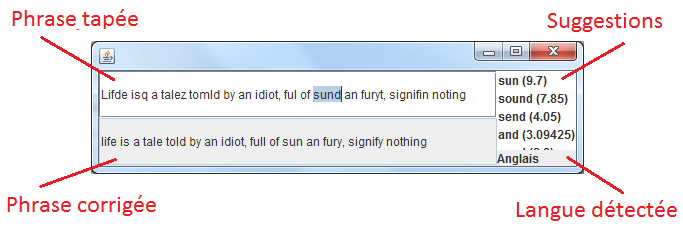
\includegraphics[scale=1.]{IHM}
\par\end{centering}
\caption{L'interface graphique montrant la correction d'une célèbre locution}
\end{figure}

La fenetre est consituée de 4 zones : \\
\begin{itemize}
\item Un champ de texte dans lequel on peut taper une phrase
\item Un champ de texte qui affiche la phrase corrigée selon notre algorithme
\item Un composant de liste, qui affiche les différentes suggestions pour le mot sélectionné et leurs probabilités
\item Un label qui affiche la langue détectée\\
\end{itemize}

Pour ne pas perturber la réactivité de l'interface, tous les calculs sont réalisés à intervalles réguliers dans un \verb!Thread! séparé. Dès qu'une modification du texte est détectée, l'ordre est donné au \verb!Thread! de mettre à jour la correction lors de sa prochaine itération.\\

Cela permet de visualiser les corrections en temps réel en conservant un sentiment de fluidité.\\

Le code source de l'interface graphique est le suivant : 

\lstinputlisting{Fenetre.java}

\section{Résultats}

\subsection{Tests simples}

\begin{figure}[H]
\begin{centering}
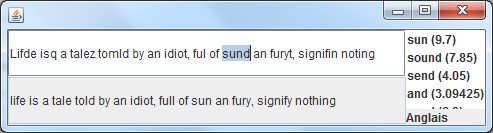
\includegraphics[scale=1.]{IHM_raw}
\par\end{centering}
\caption{Premier test, issu d'une locution bien connue}
\end{figure}

On teste notre programme avec la célèbre phrase suivante : 

\begin{quote} 
\centering 
\textit{Lifde isq a talez tomld by an idiot, ful of sund an furyt, signifin noting.}
\end{quote}

Notre programme détecte la langue anglaise, et corrige la phrase de cette manière : 

\begin{quote} 
\centering 
\textit{Life is a tale told by an idipt, full of sun an fury, signify nothing.}\\
\end{quote}

On constate que trois mots seulement sont mal corrigés.\\

\begin{itemize}
\item Le mot \textit{sund} est corrigé en \textit{sun} au lieu de \textit{sound}.\\
Examinons les suggestions et leurs probabilités : 
\begin{enumerate}
\item sun (9.7)
\item sound (7.85)
\item send (4.05)
\item and (3.09)
\item sund (2.0)
\end{enumerate}
On observe que \textit{sun}, \textit{sound} et \textit{send} sont tous trois à une distance de 1 de \textit{sund}. Ils sont donc classés par nombre d'occurrences, et le mot correct \textit{sound} n'apparait qu'en deuxième car il a été rencontré moins souvent.

De plus, la correction \textit{and} est proposée malgré le fait qu'il nécessite 2 opérations, du fait de sa très grande fréquence en anglais. Sa probabilité est du même ordre de grandeur que celles des première suggestions, mais c'est cette fois le terme du modèle de langage qui est prépondérant et non plus celui du modèle d'erreur.

Enfin, le mot \textit{sund} a été rencontré une fois seulement dans le corpus de texte. Comme c'est le mot original, cela suffit pour qu'il conserve une probabilité assez élevée.\\

\item Le mot \textit{an} est corrigé en \textit{an} au lieu de \textit{and}.\\
Examinons les suggestions et leurs probabilités
\begin{enumerate}
\item an (2047.0)
\item and (1237.0)
\item a (843.5)
\item in (640.0)
\item as (306.3)
\end{enumerate}
Le mot original \textit{an} est un mot existant, et qui plus est ayant une forte fréquence. La suggestion (correcte) \textit{and} est à nouveau proposée en deuxième, du fait de sa forte fréquence. Les mots \textit{a}, \textit{in} et \textit{as} sont tous trois également à une distance de 1, et sont donc classés par fréquence.\\

\item Le mot \textit{signifin} est corrigé en \textit{signify} au lieu de \textit{signifying}.\\
Examinons les suggestions et leurs probabilités
\begin{enumerate}
\item signify (0.00175)
\item signifying (7.5E-4)
\item signifies (6.25E-4)
\item signified (6.25E-4)
\item signifier (2.5E-4)
\end{enumerate}
Le mot original \textit{signify} sort en premier car il est plus proche du mot original. La bonne correction \textit{signifying} est encore une fois en deuxième position, suivi par trois autres propositions toutes à une distance de 2.\\
\end{itemize}

Examinons un autre exemple, en français cette fois : 

\begin{figure}[H]
\begin{centering}
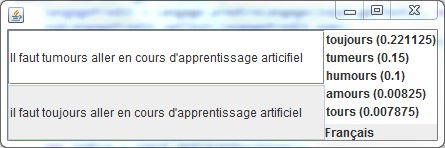
\includegraphics[scale=1.]{toujours}
\par\end{centering}
\caption{Un deuxième test, qui illustre un phénomène intéressant}
\end{figure}

La phrase entrée est

\begin{quote} 
\centering 
\textit{Il faut tumours aller en cours d'apprentissage artificiel.}
\end{quote}

Notre programme la corrige correctement ainsi : 

\begin{quote} 
\centering 
\textit{Il faut toujours aller en cours d'apprentissage artificiel.}
\end{quote}

Cet exemple est intéressant car la correction \textit{toujours} est choisie alors qu'elle est à une distance de 2, alors que la correction \textit{tumeurs} est mise de coté malgré le fait qu'elle soit plus proche du mot original, avec une distance de 1 seulement.
C'est le modèle de langage qui a permis, non pas de lever une ambiguïté entre deux mots aussi proches, mais même de prendre la décision de \textbf{favoriser un mot moins proche mais beaucoup plus fréquent}. Ce comportement est plus efficace que de simplement choisir la suggestion la plus proche.

\subsection{Tests à grande échelle}

\subsubsection{L'algorithme de test}

Nous allons généraliser ce procédé de test en générant automatiquement des fautes d'orthographe via une fonction \verb!modifier! et en les corrigeant. On observe alors le taux de corrections correctes avec la fonction \verb!evaluer!.\\

Le code-source du test est le suivant : 

\begin{lstlisting}
/**
 * Effectue une modification sur un mot, pour generer une faute
 * @param mot
 * @return
 */
public String modifier(String mot) {       
    int i = (int)(Math.random()*mot.length());
    String debut = mot.substring(0, i);
    String fin = mot.substring(i, mot.length());
    int lettre = (int)(Math.random()*alphabet.length());
    
    switch((int)(Math.random()*4)) {
    case 0: // Supression
        return debut + fin.substring(1);
    case 1: // Transposition
        if (fin.length() > 1)
            return debut + fin.charAt(1) + fin.charAt(0) + fin.substring(2);
        else return modifier(mot);
    case 2: // Mutation
        return debut + alphabet.charAt(lettre) + fin.substring(1);
    case 3: // Insertion
        return debut + alphabet.charAt(lettre) + fin;
    default:
        return mot;
    }        
}

/**
 * Evalue la performance de l'algorithme de correction
 * @param texte Un texte 
 * @param nombreMotsMax Le nombre de mots a traiter au maximum
 * @param biais Le nombre de fois qu'on considere avoir deja rencontre un mot nouveau
 */
public void evaluer(String texte, int nombreMotsMax, int biais) {
    int n = 0, fautes = 0, inconnus=0;
    for (String mot:mots(texte)) {
        if (mot.length() > 4) {
            mot = mot.toLowerCase();
            n++;
            if (biais >0)
                modele.put(mot, modele.get(mot)+biais);
            String faute = modifier(mot);
            String correction = corriger(faute);
            if (!correction.equals(mot)) {
                fautes++;
                if (!modele.containsKey(mot)){
                    inconnus++;
                    //System.out.println(mot + " inconnu !");
                }
            }
            if (n>=nombreMotsMax)
                break;
            //System.out.println(faute + " ->" + correction + "(" + modele.get(correction) + "), " + mot + " attendu (" + modele.get(mot) + ")");
        }
    }
    System.out.println(fautes + " fautes sur " + n + " mots, avec " + inconnus + " inconnus (" + (100*fautes)/n + "%, " + (100*(fautes-inconnus))/(n-inconnus) + "%)");
}
\end{lstlisting}


\subsubsection{Tests en français}

Nous essayons d'abord sur une œuvre du corpus d'apprentissage, \textit{L'argent} de Émile Zola.

On obtient le résultat suivant, sur les 1000 premiers mots : 

\begin{quote} 
\centering 
\verb!120 fautes sur 1000 mots, avec 0 inconnus (12%)!
\end{quote}

On a donc \textbf{88\% d'efficacité}, ce qui est assez satisfaisant. Cependant, cela est biaisé par le fait qu'on utilise la base dont on s'est servi pour l'apprentissage. En particulier, tous les mots lus étaient déjà connus du modèle de langage (forcément...)

Essayons avec un test plus sérieux sur une oeuvre n'appartenant pas au corpus d'apprentissage, \textit{Notre Dame de Paris}, de Victor Hugo.

\begin{quote} 
\centering 
\verb!174 fautes sur 1000 mots, avec 34 inconnus (17%)!
\end{quote}

On tombe à \textbf{83\% d'efficacité}, ce qui est logique. En effet, de nombreux mots du texte n'avaient jamais été rencontrés auparavant. En particulier, on retrouve bien sûr un grand nombre de noms propres, de lieux et de personnages. Mais pas seulement, des mots courants du français n'avaient également jamais été vus auparavant.\\

Le problème semble donc provenir du modèle de langage, qui est incomplet. Pour vérifier cette hypothèse, on ajoute un \textbf{biais} au programme, afin que lorsqu'on rencontre un mot inconnu, on simule l'avoir déjà vu plusieurs fois (100 fois par exemple). Ce procédé donne le résultat suivant : 

\begin{quote} 
\centering 
\verb!111 fautes sur 1000 mots, avec 0 inconnus (11%)!
\end{quote}

Le taux de réussite remonte à \textbf{89\% d'efficacité} et on observe des performances semblables au test sur une œuvre du corpus, ce qui est logique puisqu'on simule le fait que tous les mots soient déjà connus.

\subsubsection{Tests en anglais}

On essaie enfin sur des œuvres anglaises.\\ D'abord sur une œuvre du corpus : \textit{Frankenstein or The Modern Prometheus}, de Mary Shelley. 

\begin{quote} 
\centering 
\verb!129 fautes sur 1000 mots, avec 0 inconnus (13%)!
\end{quote}

On a un résultat de \textbf{87\% d'efficacité}, proche de l'exemple du corpus français. On tente ensuite une nouvelle œuvre, \textit{The Picture of Dorian Gray} de Oscar Wilde.

\begin{quote} 
\centering 
\verb!172 fautes sur 1000 mots, avec 41 inconnus (17%)!
\end{quote}

On obtient \textbf{83\% d'efficacité}, à nouveau les performances baissent. Comme précédemment, certains mots rencontrés étaient inconnus (des noms propres, pour la plupart), et on améliore virtuellement le modèle de langage en simulant qu'on connait tous les mots avec un biais.

\begin{quote} 
\centering 
\verb!53 fautes sur 1000 mots, avec 0 inconnus (5%)!
\end{quote}

On obtient alors \textbf{95\% d'efficacité} ce qui est très élevé, mais ce résultat est bien entendu faussé par le biais. En effet, même si l'on améliorait le modèle de langage pour qu'il connaisse plus de mots, cela augmenterait également le nombre occurrences des mauvaises corrections, ce que ne fait pas notre système de biais.

\newpage
\section{Conclusion}

Ce projet nous a permis de constater que les classifieurs naïf de Bayes, bien que très simples en théorie, font preuve d'une efficacité redoutables pour traiter certains problèmes d'apparence compliquée.\\

Notre programme a un taux d'efficacité proche de supérieur à 85\% en moyenne, ce qui est plutôt satisfaisant compte tenu des nombreuses hypothèses réductrices posées dans notre étude.\\

De nombreuses pistes d'améliorations semblent envisageable :\\

\begin{itemize}
\item Le modèle d'erreur est plutôt simpliste, et il y a de nombreux moyen de l'améliorer, par exemple pour prendre compte de la distance entre les touches du clavier. Ainsi, il est plus probable qu'un E soit remplacé par une touche voisine comme le Z plutôt que par un M qui est à l'opposé du clavier. 

\item Nous aurions aussi pu améliorer notre modèle pour qu'il prenne en compte le contexte d'un mot. En effet, en lisant le mot \textit{desert} on hésite entre les corrections \textit{désert} et \textit{dessert}. L'incertitude peut être levée si on peut apprendre à repérer dans le contexte de la phrase des mots tels que \textit{sucré}, \textit{délicieux} ou bien \textit{sable}, \textit{chaleur} et en déduire des corrélations par des tests du $\xi_2$
\item Le modèle actuel ne prend pas en compte les règles de grammaire, qu'il serait très utile d'implémenter. Il paraît même envisageable, quoique compliqué, d'utiliser des algorithmes d'apprentissage pour déduire de la lecture d'un corpus de texte certaines règles de grammaire
\end{itemize}


\end{document}